
\subsection{Calamiteiten pagina}
\pvelist{ \pve{4.1.1.2, 4.4} }
Om de site in calamiteiten mode te zetten ga je als volgt te werk:

\begin{enumerate}
\item Ga naar \drupalpath{node/237/edit} om de calamiteiten pagina te bewerken indien nodig
\item Controleer of de calamiteitenpagina is gepubliceerd
\item Ga naar \emph{Structuur} $\rightarrow$ \emph{Dominion} of direct naar \drupalpath{admin/structure/dominion/list/1/edit}
\item Vul bij \emph{voorpagina} de tekst \emph{calamiteiten} in
\item Klik op Oplaan
\end{enumerate}

Op de calamiteitenpagina heeft de redacteur alle vrijheid om blokken te plaatsen, net zoals alle andere pagina's.

\begin{figure}[p]
\centering
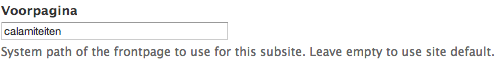
\includegraphics[width=\textwidth]{img/calamiteiten.png}
\caption{Calamiteiten pagina activeren}
\label{fig:calamiteiten_image}
\end{figure}